\section{Easy Keygen}
\begin{enumerate}
\item 运行程序,随意输入,程序结束。\\
\item IDA打开查看函数列表确认没有加壳,直接静态分析。\\
\item
	\begin{enumerate}
	\item Shift + F12  打开Strings窗口,找到字符串“\lstinline$Correct!\n$”,\\
	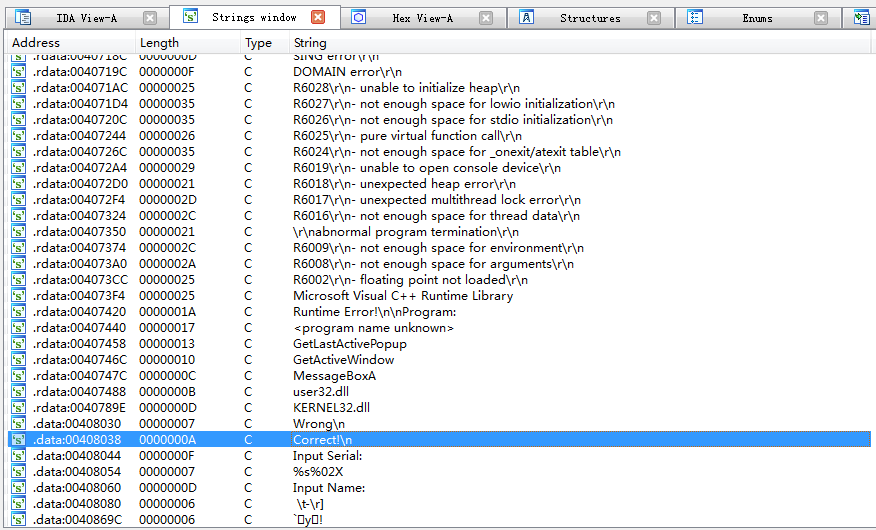
\includegraphics[width=10cm]{easykeygen-msg} \\
	\item 双击 转到字符串定义,\\
	\item 双击 交叉引用(DATA XREF)的函数名,跳转到对应函数定义,\\
	\item 空格 切换为Graph View分析函数功能 \\
	\end{enumerate} 
\item 
	分析左侧分支(红色框)会用到“\lstinline$Correct!\n$”:\\
	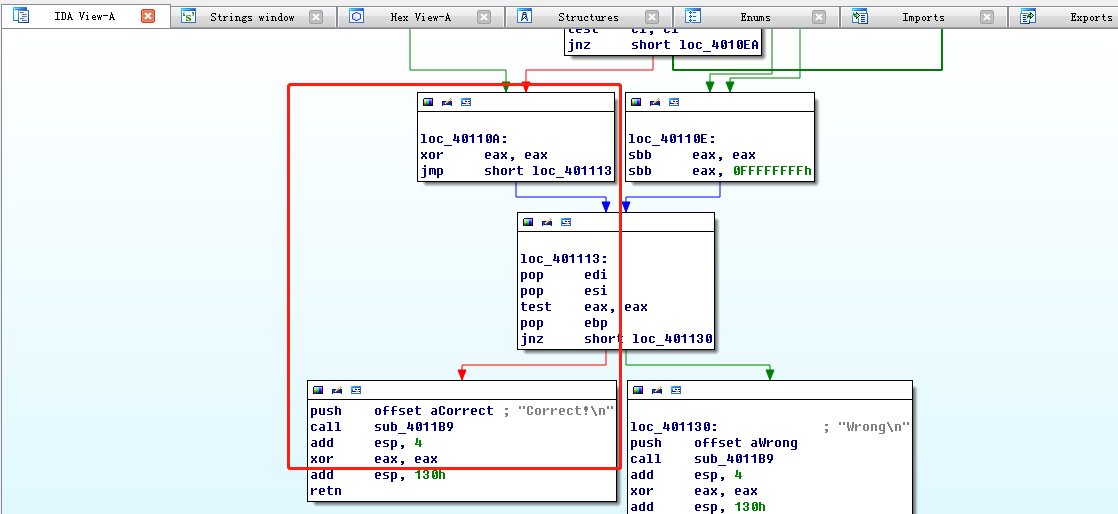
\includegraphics[width=10cm]{easykeygen-judge} \\
	分析输入存储位置: \\
	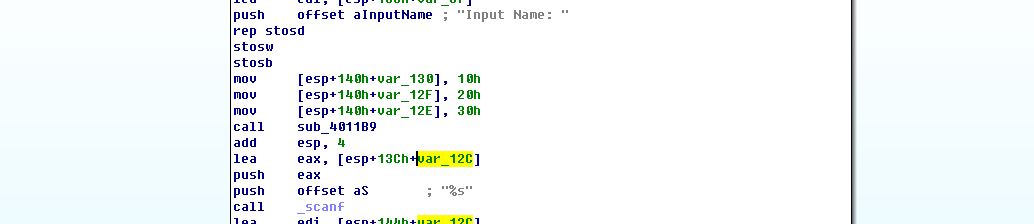
\includegraphics[width=10cm]{easykeygen-name} \\
	\lstinline$[esp+13Ch+var_12C]$为输入Name存储地址 \\
	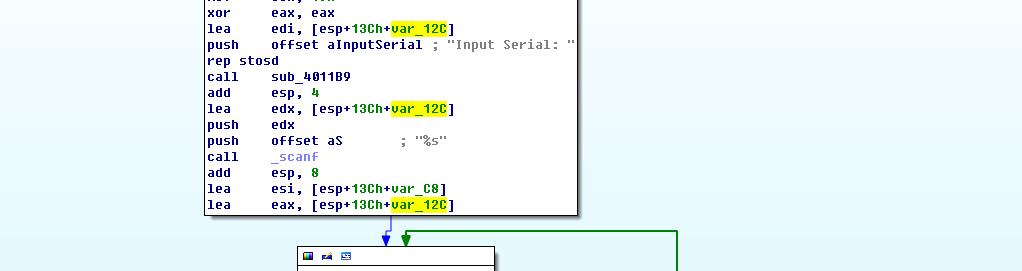
\includegraphics[width=10cm]{easykeygen-serial} \\
	\lstinline$[esp+13Ch+var_12C]$为输入Serial存储地址,紧接着 \\
	\begin{lstlisting}
	lea     esi, [esp+13Ch+var_C8]
	lea     eax, [esp+13Ch+var_12C]
	\end{lstlisting}
	经过分析,后面的代码是在比较两个字符串是否相等,\\
	\lstinline$[esp+13Ch+var_12C]$为刚刚输入的Serial,\\
	\lstinline$[esp+13Ch+var_C8]$应该就是输入的Name经过某些处理(算法)得到的Serial值 \\
	输入Name与输入Serial之间的代码,即为Name转换为Serial的算法,着重分析即可:\\
	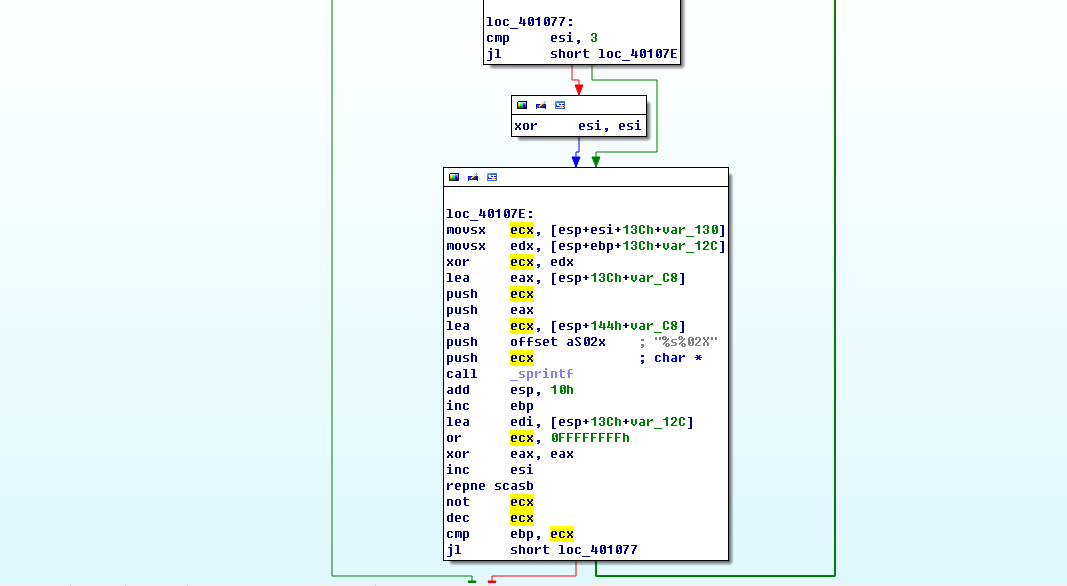
\includegraphics[width=10cm]{easykeygen-alg} \\
	将输入Name的每个字节依次与\lstinline$[esp+esi+13Ch+var_130]$存储的3个字节  \\
	进行异或操作,并格式化为2位16进制格式存储至\lstinline$[esp+13Ch+var_C8]$ \\
	\begin{lstlisting}
	mov     [esp+140h+var_130], 10h
	mov     [esp+140h+var_12F], 20h
	mov     [esp+140h+var_12E], 30h
	\end{lstlisting}
	\lstinline$[esp+esi+13Ch+var_130]$存储的3个字节为:10h、20h、30h \\
	将Serial : ``5B134977135E7D13''两两分组,依次分别与10h、20h、30h异或,\\
	然后转换为字符 \\
	\begin{lstlisting}
	#include <stdio.h>
	int main()
	{
		int salt[3] = { 0x10, 0x20, 0x30 };
		char serial[8] = { 0x5B, 0x13, 0x49, 0x77, 0x13, 0x5E, 0x7D, 0x13 };
		int i = 0;
		for (i = 0; i < 8; i++)
			printf("%c",  serial[i] ^ salt[i % 3]);
		printf("\n");
	}
	\end{lstlisting}
	flag : ``K3yg3nm3''

\end{enumerate}